\documentclass[a4paper, 11pt,reqno]{article}
\input{/Users/olivierglorieux/Desktop/BCPST/2020:2021/preambule.tex}
\newif\ifshow
\showfalse
%\geometry{hmargin=3cm,vmargin=4cm }
\input{/Users/olivierglorieux/Desktop/BCPST/2021:2022/ifshow.tex}


\author{Olivier Glorieux}


\begin{document}

\title{DM8
}


Le but de ce DM est de calculer la valeur de 
$$\lim_{n\tv \infty} \sum_{k=1}^n \frac{1}{k^2}$$

\paragraph{Convergence}
On note $S_n=  \sum_{k=1}^n \frac{1}{k^2}$.

\begin{enumerate}
\item Montrer que la suite $\suite{S}$  est monotone. 
\item Montrer que pour tout $k\geq 2$
$$\frac{1}{k^2} \leq \frac{1}{k-1}-\frac{1}{k}$$
\item En déduire que la suite $\suite{S}$ converge vers une limite $\ell \in [0,2]$. 
\end{enumerate}

\begin{correction}
\begin{enumerate}
\item Pour tout $n\in \N$ on a  $S_{n+1} = S_n + \frac{1}{(n+1)^2}$, donc 
$S_{n+1}-S_n = \frac{1}{(n+1)^2}\geq 0$. Ainsi, $\suite{S}$ est croissante. 
\item Pour tout $k\geq 2$ : $\frac{1}{k-1}-\frac{1}{k}= \frac{k-(k-1)}{k(k-1)}= \frac{1}{k(k-1)}$
Or pour tout $k\geq 2$,  $0<k(k-1) \leq k^2$. Comme la fonction inverse est décroissante sur $\R_+^*$ on a donc : 
$$\frac{1}{k-1}-\frac{1}{k}=\frac{1}{k(k-1)}\geq \frac{1}{k^2}$$

\item  D'après la question précédente, on peut majorer tous les termes de $S_n$ à partir du rang $k=2$. On  a alors : 
$$S_n = 1+ \sum_{k=2}^n\frac{1}{k^2} \leq 1 + \sum_{k=2}^n\frac{1}{k-1} -\frac{1}{k}$$
On reconnait alors dans le  membre de droite une somme téléscopique qui se simplifie de la manière suivante : 
$$\sum_{k=2}^n\frac{1}{k-1} -\frac{1}{k} = \frac{1}{2-1} -\frac{1}{n} = 1-\frac{1}{n}$$
On obtient alors $S_n  \leq 2-\frac{1}{n}$. 
La suite $\suite{S}$ est croissante et majorée, d'après le théorème des limlites monotones la suite $\suite{S}$ converge, notons $\ell$ sa limite. 

Comme $0\leq S_n\leq 2-\frac{1}{n}$ et $\lim_{n\tv \infty} 2-\frac{1}{n}=2$, le théorème d'encadrement assure que $\ell\in [0,2]$. 
 


\end{enumerate}
\end{correction}






\paragraph{Calcul de la limite}
Pour tout $n\in \N$ on définit $I_n$ et $J_n$ par 
$$I_n = \int_0^{\frac{\pi}{2}} \cos^{2n}(t) dt \quad J_n=\int_0^{\frac{\pi}{2}} t^2 \cos^{2n}(t) dt$$
\begin{enumerate}
\item Montrer que $I_0= \frac{\pi}{2}$ et $J_0 = \frac{\pi^3}{24}$
\item \begin{enumerate}
\item En utilisant une intégration par parties, démontrer que pour tout entier $n\geq 1$ on a :
$$I_n =\frac{2n-1}{2n} I_{n-1}$$
(on pourra utiliser que $\cos^{2n}(t)=\cos^{2n-1}(t)\cos(t)$)
\item En déduire que 
$$I_n = \frac{(2n)! }{2^{2n} (n!)^2} \frac{\pi}{2}$$
\end{enumerate}
\item \begin{enumerate}
\item En utilisant une intégration par parties, montrer que : 
$$\int_0^{\frac{\pi}{2}} t \cos^{2n-1}(t)\sin(t) dt =\frac{1}{2n} I_n$$
\item Montrer que $$J_{n-1} -J_n = \int_0^{\frac{\pi}{2}}( t^2 \sin(t)) \cos^{2n-2}(t)\sin(t) dt$$
\item En utilisant une intégration par parties en déduire que :
$$J_{n-1} -J_n = \frac{1}{2n-1}\left( \frac{1}{n}I_n +J_n\right)$$
\item On désigne par $\suite{K}$ la suite réelle définie par $K_n = \frac{J_n}{I_n}$. 
En utilisant la relation obtenue précédemment, montrer que :
$$\frac{J_{n-1}}{I_n} -K_n = \frac{1}{2n-1}\left( \frac{1}{n} +K_n\right)$$
puis en déduire que :
$$K_{n-1} - K_n =\frac{1}{2n^2}$$
\end{enumerate}
\item Le but de cette question est de montrer que $K_n \tv 0$ 
\begin{enumerate}
\item démontrer que pour tout réel $t\in [0, \frac{\pi}{2}] $ on a :
$$t\leq \frac{\pi}{2 }\sin(t)$$
\item  En déduire que pour tout entier $n$ on  a: 
$$0\leq J_n \leq \frac{\pi^2 I_n}{8(n+1) }$$
puis que : 
$$0\leq K_n \leq \frac{\pi^2 }{8(n+1) }$$
\end{enumerate}
\item En déduire que $$\lim_{n\tv \infty} S_n =\frac{\pi^2}{6}$$
\end{enumerate}


\begin{correction}
\begin{enumerate}
\item Calculons $I_0$ et $J_0$
 $$I_0  = \int_0^{\frac{\pi}{2}} \cos^{0}(t) dt = \int_0^{\frac{\pi}{2}} 1dt= \left[t \right]_0^{\frac{\pi}{2}} =\frac{\pi}{2}$$
et 
 $$J_0  = \int_0^{\frac{\pi}{2}} t^2\cos^{0}(t) dt = \int_0^{\frac{\pi}{2}} t^2dt= \left[\frac{t^3}{3} \right]_0^{\frac{\pi}{2}} =\frac{\pi^3}{8*3}=\frac{\pi^3}{24}$$
\item 
\begin{enumerate}
\item 

On utilise l'intégration par partie proposée dans l'indication : 
$$I_n  =  \int_0^{\frac{\pi}{2}}  \cos(t) \cos^{2n-1} (t) dt $$
on pose $u'(t)= \cos(t) $ et $v(t) =\cos^{2n-1}(t)$. On a $u(t)= \sin(t)$ et $v'(t) = -(2n-1) \sin(t) \cos^{2n-2}(t)$. On obtient alors : 
\begin{align*}
I_n &= \left[ \sin(t) \cos^{2n-1}(t)\right]_0^{\frac{\pi}{2}}  +(2n-1) \int_0^{\frac{\pi}{2}}  \sin^2(t) \cos^{2n-2} (t)dt
\end{align*}
Le crochet $\left[ \sin(t) \cos^{2n-1}(t)\right]_0^{\frac{\pi}{2}}$ est nul et on utilise la relation $\cos^2(t) + \sin^2(t) =1$ pour l'intégrale de droite : 
$\int_0^{\frac{\pi}{2}}  \sin^2(t) \cos^{2n-2} (t)dt =  \int_0^{\frac{\pi}{2}}  \cos^{2(n-1)} (t)- \cos^{2n}(t)dt = I_{n-1} -I_n$
Grâce au calcul précédent on obtient : 
$$I_n = (2n-1)(I_{n-1} -I_n)$$ 
soit encore $2nI_n = (2n-1) I_{n-1}$ ce qui donne le résultat voulu en divisant par $2n$. 

\item On peut prouver le résultat par récurrence.  La formule est vraie au rand 0 d'après la question 1. On la suppose vraie à un rang n fixé. D'après la question précédente, on a : 
\begin{align*}
I_{n+1} &= \frac{2n+1}{2(n+1)} I_{n}
\end{align*}
Par hypothèse de récurrence,  $I_n =  \frac{(2n)! }{2^{2n} (n!)^2} \frac{\pi}{2}$, donc 

\begin{align*}
I_{n+1} &= \frac{2n+1}{2(n+1)} \frac{(2n)! }{2^{2n} (n!)^2} \frac{\pi}{2}
\end{align*}
Enfin, en multipliant en haut et en bas par $(2n+2)$ on obtient : 
\begin{align*}
\frac{2n+1}{2(n+1)} \frac{(2n)! }{2^{2n} (n!)^2}  &=  \frac{2n+2}{2n+2}\frac{2n+1}{2(n+1)} \frac{(2n)! }{2^{2n} (n!)^2} \\
&= \frac{(2(n+1))!}{ 2*2 (n+1)^2 (2^{2n} (n!)^2)}\\
&= \frac{(2(n+1))!}{ 2^{2n+2} ((n+1)!)^2}
\end{align*}
La formule est donc vérifiée au rang $(n+1)$ ; par principe de récurrence la formule est vraie pour tout $n\in \N$. 

\end{enumerate}
\item 
\begin{enumerate}
\item 
Refaisons une intégration par partie, en posant cette fois 
$u'(t)= 1 $ et $v(t) =\cos^{2n}(t)$. On a $u(t)= t$ et $v'(t) = -2n \sin(t) \cos^{2n-1}(t)$. On obtient alors : 
\begin{align*}
I_n &= \left[ t \cos^{2n}(t)\right]_0^{\frac{\pi}{2}}  +(2n) \int_0^{\frac{\pi}{2}}  t \sin(t) \cos^{2n-1} (t)dt
\end{align*}
De nouveau le crochet est nul. En divisant par $2n$ on obtient bien l'égalité demandée. 
\item Poru tout $n\in \N$ on a 
\begin{align*}
J_{n-1}-J_n &= \int_0^{\frac{\pi}{2}} t^2 \cos^{2(n-1)}(t) dt- \int_0^{\frac{\pi}{2}} t^2 \cos^{2n}(t) dt\\
&=\int_0^{\frac{\pi}{2}} t^2 \cos^{2n-2}(t)(1-\cos^2(t)) dt\\
&=\int_0^{\frac{\pi}{2}} t^2 \sin^2(t)\cos^{2n-2}(t)dt
\end{align*}
Ce qui correspond à la formule demandée, à permutation prés d'un $\sin(t)$.

\item La formule proposée dans la question précédente laisse penser à poser les fonctions suivantes pour l'intégration par parties :  
 $u'(t)= \sin(t)\cos^{2n-2}(t) $ et $v(t) =t^2\sin(t)$. On a $u(t)= \frac{-1}{2n-1}\cos^{2n-1}(t)$ et $v'(t) =2t\sin(t) +t^2 \cos(t)$. Ainsi :
 \begin{align*}
 J_{n-1}-J_n&= \left[ t^2  \sin(t) \frac{-1}{2n-1}\cos^{2n-1}(t)\right]_0^{\frac{\pi}{2}}   + \frac{1}{2n-1} \int_0^{\frac{\pi}{2}} \cos^{2n-1}(t)(2t\sin(t) +t^2 \cos(t))dt
 \end{align*}
Encore une fois, le crochet est nul et 
\begin{align*}
\int_0^{\frac{\pi}{2}} \cos^{2n-1}(t)(2t\sin(t) +t^2 \cos(t))dt &= \int_0^{\frac{\pi}{2}} \cos^{2n-1}(t)(2t\sin(t)) +t^2 \cos^{2n}(t)dt\\
&=2 \int_0^{\frac{\pi}{2}} t\cos^{2n-1}(t)\sin(t) +J_n\\
&= \frac{1}{n}I_n +J_n
\end{align*}
Où la dernière ligne est obtenue à l'aide de la formule de la quesiton 3a). 
Avec l'équation précédente, on a alors : 
\begin{align*}
J_{n-1} -J_n &= \frac{1}{2n-1} \left(  \frac{1}{n}I_n +J_n \right)
\end{align*}
\item 
Il suffit de diviser par $I_n$ (qui est non nul d'après la question 2b)) la relation précédente   
\begin{align*}
\frac{1}{I_n}(J_{n-1} -J_n) &= \frac{1}{I_n} \left(\frac{1}{2n-1} \left(  \frac{1}{n}I_n +J_n \right)\right)\\
\frac{J_{n-1}}{I_n} -K_n &=  \frac{1}{2n-1} \left(  \frac{1}{n} +K_n \right)
\end{align*}
\item 
\begin{align*}
\frac{J_{n-1}}{I_n} &= \frac{J_{n-1} I_{n-1}}{I_n I_{n-1}} \\
							&= \frac{K_{n-1} I_{n-1}}{I_n } \\	
							&= \frac{2n K_{n-1}}{2n-1 } 
\end{align*}
où la dernière égalité est obtenue avec la formule de la question 2a). On  a alors : 

\begin{align*}
\frac{2n K_{n-1} }{2n-1 }  - K_n &= \frac{1}{2n-1} \left(  \frac{1}{n} +K_n \right)\\
2n K_{n-1}  - (2n-1) K_n &=  \left(  \frac{1}{n} +K_n \right)\\
 2n(K_{n-1} -K_n) &= \frac{1}{n}\\
 K_{n-1}- K_n &= \frac{1}{2n^2}
\end{align*}




\end{enumerate}

\item \begin{enumerate}
\item On  va étudier al fonction $f(t) = t- \frac{\pi}{2} \sin(t)$ sur $I=[0,\frac{\pi}{2}]$. Cette fonction est bien définie est dérivable sur cet intervalle et on  a : $f'(t)=1 -\frac{\pi}{2}\cos(t)$
Comme $\cos$ est strictement décroissant sur $I$, que $f'(0) =1-\frac{\pi}{2}<0$ et $f'(\frac{\pi}{2}) =1-0=1>0 $, il existe un unique $\alpha\in I$ tel que $f'(x)<0 $ sur $[0,\alpha]$ et $f'(x)\geq 0 $ sur $[\alpha,\frac{\pi}{2}]$. 

On obtient le tableau de variations suivants : 

\begin{center}
\begin{tikzpicture}
\tkzTabInit[espcl=6]{$x$ / 1,Signe de\\$f'(x)$/1, Variations de\\ $f$ / 3}%
{$0$, $\alpha$, $\frac{\pi}{2}$}%
\tkzTabLine{,-,0,+, }
\tkzTabVar{+/$0$ , -/$f(\alpha)$,+/$0$ }
   \end{tikzpicture}
\end{center}
 
 On voit alors que $f(t)\leq 0$ pour tout $t\in I$ ce qui revient bien à 
 $$ \forall t \in  I, 
 \, t\leq \frac{\pi}{2 }\sin(t)$$
\item Sur $I$ on a $0\leq t \leq  \frac{\pi}{2 }\sin(t)$, en mettant au carré on obtient $$t^2 \leq  \frac{\pi^2}{4 }\sin^2(t)$$, ainsi 
$$J_n \leq \int_0^{\frac{\pi}{2}}   \frac{\pi^2}{4 }\sin^2(t) \cos^{2n}(t) dt$$
D'où en utilisant une n-iéme fois $\cos^2+\sin^2=1$ :
$$J_n \leq \frac{\pi^2}{4 }  \int_0^{\frac{\pi}{2}}   \cos^{2n}(t) - \cos^{2n+2}(t)   dt  = \frac{\pi^2}{4} (I_n-I_{n+1})$$
En utilisant la quetison 2a) on a :
$I_{n+1} = \frac{2n+1}{2(n+1)}I_n$ 
Donc 
\begin{align*}
J_n &\leq  \frac{\pi^2}{4} I_n \left( 1 - \frac{2n+1}{2(n+1)}\right)\\
			&\leq  \frac{\pi^2}{4} I_n \left(   \frac{2(n+1)- 2n+1}{2(n+1)}\right)\\
			&\leq  \frac{\pi^2}{4} I_n  \frac{1}{2(n+1)}\\
			&\leq  \frac{\pi^2}{8(n+1)} I_n  
\end{align*}
Par ailleurs $J_n\geq 0$ car $t^2 \cos^n(t)\geq 0$  pour tout $t\in I$. 
En divisant de par et d'autre par $I_n$ on  obtient 
$$0\leq K_n \leq   \frac{\pi^2}{8(n+1)} $$

Or $\lim_{n\tv +\infty}  \frac{\pi^2}{8(n+1)} =0$ 
D'après le théorème des gendarmes, $\suite{K}$ converge et sa limite vaut $0$. 

\end{enumerate}
\item D'après la question 3d)  $\sum_{j=1}^n  K_{j-1} -K_j =\sum_{j=1}^n \frac{1}{2 j^2}$
On reconnait $\frac{1}{2}S_n$ dans le membre de droite et une somme telescopique dans la somme de gauche, on obtient donc : 
$$K_{0}-K_n =\frac{1}{2} S_n$$
Enfin $K_0 =\frac{J_0}{I_0} = \frac{\pi^3 2}{24 \pi} = \frac{\pi^2}{12}$
D'où 
$$S_n = \frac{\pi^2}{6} -2K_n.$$
Commet $K_n\tv 0$ quand $n\tv +\infty$, on  a bien ; 
$$ \lim_{n\tv \infty} S_n  =\frac{\pi^2}{6}$$




\end{enumerate}
\end{correction}

\end{document}